\documentclass[a4paper,10pt,oneside]{article}
\usepackage{epsfig}
\usepackage{color}
\usepackage{url}
\usepackage[utf8]{inputenc}
\usepackage[T1]{fontenc}
\usepackage{amsmath}
\usepackage{amssymb}
\usepackage{import}

\newcommand{\myscale}{0.74}
\newcommand{\vect}[1]{\boldsymbol{#1}}
\newcommand{\code}[1]{\texttt{#1}}

\setlength{\hoffset}{-1in} %left margin will be 0, as hoffset is by default 1inch
\setlength{\voffset}{-1in} %analogous voffset
\setlength{\oddsidemargin}{1.5cm}
\setlength{\evensidemargin}{1.5cm}
\setlength{\topmargin}{1.5cm}
\setlength{\textheight}{26cm}
\setlength{\textwidth}{18cm}




\def\mftitle{jInfer Architecture}
\def\mfauthor{Michal Klempa, Mário Mikula, Robert Smetana, Michal Švirec, Matej Vitásek}
\def\mfadvisor{RNDr. Irena Mlýnková, Ph.D., Martin Nečaský, Ph.D.}
\def\mfplacedate{Praha, 2011}
\title{\bf\mftitle}
\author{\mfauthor \\ Advisors: \mfadvisor}
\date{\mfplacedate}

\ifx\pdfoutput\undefined\relax\else\pdfinfo{ /Title (\mftitle) /Author (\mfauthor) /Creator (PDFLaTeX) } \fi

\begin{document}
\maketitle
Target audience: developers willing to extend jInfer.\\

\textit{Note: we use the term \textbf{inference} for the act of creation of schema throughout this and other jInfer documents.}\\

The description of jInfer architecture will commence by describing the data
structures, namely representations of regular expressions and XML elements,
attributes and simple data.

Afterwards the interfaces of basic inference modules - Initial Grammar Gen-
erator, Simplifier and Schema Generator - will be explained.

Finally, the process of inference will be described.

\section{Package naming conventions}
All packages start with \code{cz.cuni.mff.ksi.jinfer}. Afterwards is the short, normalized name of the module (e.g. \code{base}) and finally the package structure in this module (e.g. \texttt{objects.utils}). All in all, a package in the Base module could look like 
\code{cz.cuni.mff.ksi.jinfer.base.objects.utils}

\section{Data structures}
\subsection{Regular expressions}

For general information on regular expressions, please refer to \cite{wikiregexp}, \cite{automatatheory}.
All classes pertaining to regular expressions can be found in the package \code{cz.cuni.mff.ksi.jinfer.base.regexp}.
In jInfer, we use extended regular expressions as they give us nicer syntax (and easier programming).

Regular expression is implemented as class \code{Regexp} with supplementing classes \code{RegexpInterval} and \code{RegexpType}.
Each \code{Regexp} instance has one of the enum \code{RegexpType} type:
\begin{itemize}
	\item Lambda - empty string (also called $\epsilon$ in literature),
	\item Token - a letter of the alphabet,
	\item Concatenation - one or more regular expression in an ordered sequence. Eg. $(a, b, c, d)$,
	\item Alternation - a choice between one or more regular expressions. Eg. $(a | b | c | d)$,
	\item Permutation - shortcut for all possible permutations of regular expressions. Our syntax to write down permutation is $(a\& b\& c\& d)$.
\end{itemize}

Each \code{Regexp} instance has one instance of \code{RegexpInterval} as member.
Class \code{RegexpInterval} represents POSIX-like intervals for expression:
\begin{itemize}
	\item $a\{m,n\}$ means $a$ at least $m$-times, at most $n$-times,
	\item $a\{m,\}$ means at least $m$-times (unbounded).
\end{itemize}

Class \code{Regexp} can represent regular expression over any alphabet.
This is done by using java generics, \code{Regexp} is implemented as \code{Regexp<T>}.
Regular expression is in fact $n$-ary tree, for example expression $(a, b, (c | d))$ can be viewed as in figure \ref{reg:tree}.
\begin{figure}
\caption{Example tree for regular expression $(a, b, (c | d))$} \label{reg:tree}
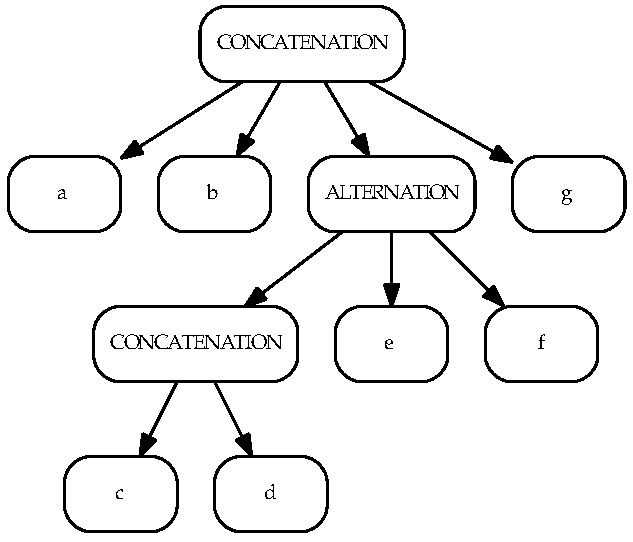
\includegraphics[scale=1]{reg_tree}
\end{figure}

\nocite{*}
\bibliographystyle{alpha}
\bibliography{literature}

\end{document}
